\documentclass[11pt,a4paper]{article}
\usepackage[margin=18mm,headheight=14pt]{geometry}
\usepackage[T1]{fontenc}
\usepackage[utf8]{inputenc}
\usepackage{lmodern,microtype,amsmath,amssymb,booktabs,array,xcolor,fancyhdr,graphicx}
\usepackage[most]{tcolorbox}
\usepackage{pgfplots}
\pgfplotsset{compat=1.18}
\usepackage[colorlinks=true,urlcolor=blue]{hyperref}
\definecolor{ink}{HTML}{17334C}
\definecolor{pale}{HTML}{EEF4F7}
\definecolor{rust}{HTML}{A64B2A}
\setlength{\parindent}{0pt}
\setlength{\parskip}{6pt}
\pagestyle{fancy}\fancyhf{}
\fancyhead[L]{\small\color{ink} PERFIL RADIAL E ESTRUTURA ESPECTRAL}
\fancyhead[R]{\small 28.09.2026}
\fancyfoot[L]{\footnotesize Mauro de Oliveira Cardoso (Viole) | Material para discussão}
\fancyfoot[R]{\thepage/6}
\renewcommand{\headrulewidth}{0.3pt}
\newcommand{\titlepageof}[3]{\vspace*{2mm}{\small\color{rust}\textbf{#1}}\par
 {\LARGE\bfseries\color{ink}#2}\par{\large #3}\par\vspace{2mm}}
\newtcolorbox{panel}[1]{colback=pale,colframe=ink,boxrule=0.4pt,arc=1mm,
 title={#1},fonttitle=\bfseries,coltitle=white,left=3mm,right=3mm,top=2mm,bottom=2mm}
\newcommand{\source}[1]{\vfill{\footnotesize\raggedright\color{ink}\textbf{Fonte local:} #1\par}}
\newcommand{\M}{M_*}
\begin{document}
\titlepageof{01 / PERGUNTA CENTRAL}{O que a forma do perfil revela?}{Da quebra de uma simetria de 1-forma ao limiar acoplado}
Uma simetria elétrica de 1-forma permite medir carga por uma superfície que
envolve uma linha de prova. Com matéria carregada, o screening faz a carga
efetiva $q(r)$ depender do raio. A pergunta é: \textbf{quanto do espectro pode
ser inferido dessa dependência?}
\begin{panel}{O observável e sua representação condicional}
\begin{equation*}
 \delta(r)=-\frac{r}{q_\infty}q'(r),\qquad \Phi(r)=\frac{\delta(r)}{r^2},
 \qquad q_\infty\ne0.
\end{equation*}
\begin{equation*}
 \Phi(r)=\int_{\M}^\infty e^{-rx}\,d\nu(x),\qquad
 d\nu\ge0,\quad \M=\inf\operatorname{supp}\nu.
\end{equation*}
$x=\sqrt{s}$ tem dimensão de massa. A medida $\nu$ contém o peso com que
cada massa contribui a este observável; não é uma contagem de partículas.
\end{panel}
\begin{center}\small
Resposta estática positiva (H3)\\[2pt]
$\Downarrow$\\[-1pt]
Perfil reduzido como transformada de Laplace\\[2pt]
$\Downarrow$\\[-1pt]
Momentos positivos $\longrightarrow$ limites superiores para o limiar
\end{center}
\begin{equation*}
 \Gamma(r)=-\partial_r\log\Phi(r)=\langle x\rangle_r\ge\M,
 \qquad \Gamma'(r)=-\operatorname{Var}_r(x)\le0.
\end{equation*}
\textbf{Estabelecido condicionalmente.} Para medida não nula, com as condições
de integrabilidade do artigo, $\Gamma(r)$ decresce para a borda efetiva do
suporte. A técnica de effective mass e GEVP é clássica.

\textbf{Interpretação correta.} $\M$ é o menor limiar \emph{acoplado ao
observável}. Identificá-lo com a menor massa carregada exige informação de
canal. No exemplo de um laço de Dirac, o limiar de par é $2m$, não $m$.

\begin{panel}{Questão aberta principal}
A QFT garante a H3 para o kernel estático invariante de gauge no regime
pretendido? A positividade de um correlacionador de dois campos não fecha,
sozinha, essa passagem.
\end{panel}
\source{\texttt{paper/paper.tex}, hipóteses H1--H5 e teoremas A, C, E.
Unidades $\hbar=c=1$; resposta linear a uma fonte infinitamente pesada.}
\newpage
\titlepageof{02 / HIPÓTESE FÍSICA}{Positividade: onde está a lacuna?}{H3 é uma entrada física, não uma conclusão dos testes}
\begin{panel}{H3 na formulação canônica}
\begin{equation*}
 \mathcal G(Q^2)=\frac{g_R^2}{Q^2}
 +\int_{s_*}^\infty\frac{d\sigma(s)}{Q^2+s},\qquad d\sigma\ge0.
\end{equation*}
$Q^2=|\mathbf p|^2>0$, $g_R^2>0$, $s_*>0$ e
$\int d\sigma(s)/(\mu_0^2+s)<\infty$ para alguma escala $\mu_0>0$.
A expressão não inclui um termo polinomial de contato.
\end{panel}
\textbf{O que se segue.} O transformado de Yukawa e a lei de Gauss dão,
em resposta linear,
\begin{equation*}
 \int f(x)\,d\nu(x)=\frac{1}{g_R^2}\int s\,f(\sqrt{s})\,d\sigma(s).
\end{equation*}
Essa definição também vale para átomos. A identidade
$[(1+r\sqrt{s})e^{-r\sqrt{s}}]'=-sr e^{-r\sqrt{s}}$ produz o perfil reduzido.

\textbf{O que existe a ordem líder.} A positividade de Lehmann da corrente
da matéria \emph{não gaugeada}, com a relação de dispersão subtraída adotada,
fornece a contribuição espectral positiva a um laço. Não é uma prova para
a autoenergia 1PI completa nem para o potencial não perturbativo.

\begin{panel}{Três etapas que não devem ser confundidas}
\textbf{1. Correlacionador.} Wightman, covariância de Lorentz e Bianchi
restringem $\langle FF\rangle$. No cone de luz, a eliminação do termo
helicoidal também usa localidade via CPT, ainda pendente de leitura na nota.

\textbf{2. Observável estático.} É preciso controlar o laço de Wilson,
renormalização de perímetro, contatos e o limite $T\to\infty$.

\textbf{3. Regime físico.} Fase de Coulomb, resposta linear e eventual gap
são hipóteses adicionais. Um canal sem massa pode destruir o gap sem
destruir a positividade.
\end{panel}
\textbf{Atualização desta rodada.} O critério exploratório $Z_3\ge0$ exige
cuidado: a classe geral de Stieltjes permite uma constante. Há um
contraexemplo exato à equivalência direta com H3 na fronteira $Z_3=0$
(backup, p.~6).

\begin{panel}{Pergunta para o professor}
Que hipóteses adicionais permitem transportar a medida positiva de
$\langle FF\rangle$ ao coeficiente de resposta linear do laço de Wilson,
controlando contatos e o limite estático, sem presumir a própria H3?
\end{panel}
\source{\texttt{paper/appendix.tex}; \texttt{notes/E2b\_tensor\_classification.tex};
\texttt{reports/H3\_BOUNDARY\_CORRECTION\_2026-09-28.md}.}
\newpage
\titlepageof{03 / CONTRAEXEMPLO}{Um estado leve quase invisível}{Um limite válido pode continuar pouco informativo}
Considere a medida positiva, em unidades fixadas pelo modelo,
\begin{equation*}
 d\nu(x)=10^{-12}\delta_2(dx)+(x-3)^{1/2}e^{-(x-3)}\mathbf1_{x\ge3}\,dx.
\end{equation*}
A borda verdadeira é $\M=2$, mas o contínuo começa em $3$. A transformada é
\begin{equation*}
 \Phi(r)=\underbrace{10^{-12}e^{-2r}}_{\text{átomo leve}}
 +\underbrace{\Gamma_E(3/2)(1+r)^{-3/2}e^{-3r}}_{\text{contínuo}}.
\end{equation*}
\begin{center}
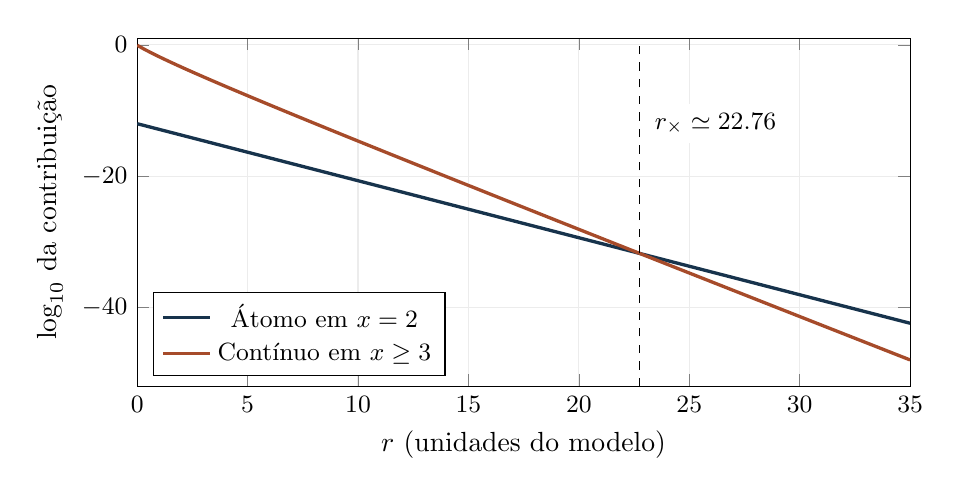
\begin{tikzpicture}
\begin{axis}[width=0.94\linewidth,height=6cm,xmin=0,xmax=35,ymin=-52,ymax=1,
 xlabel={$r$ (unidades do modelo)},ylabel={$\log_{10}$ da contribuição},
 grid=major,grid style={gray!15},legend style={font=\small,at={(0.02,0.03)},anchor=south west},
 tick label style={font=\small}]
\addplot[ink,very thick,domain=0:35,samples=100]{-12-2*x/ln(10)};
\addlegendentry{Átomo em $x=2$}
\addplot[rust,very thick,domain=0:35,samples=100]{ln(0.88622692545)/ln(10)-1.5*ln(1+x)/ln(10)-3*x/ln(10)};
\addlegendentry{Contínuo em $x\ge3$}
\draw[dashed] (axis cs:22.758,-52)--(axis cs:22.758,1);
\node[anchor=west,font=\small,fill=white] at (axis cs:23,-12){$r_\times\simeq22.76$};
\end{axis}
\end{tikzpicture}
\end{center}
\textbf{Crossover deste modelo:}
$10^{-12}e^{r_\times}=\Gamma_E(3/2)(1+r_\times)^{-3/2}$.
Numericamente, $\Gamma(10)\simeq3.136$, $\Gamma(20)\simeq3.018$ e
$\Gamma(30)\simeq2.0005$. São verificações numéricas, não dados experimentais.

\begin{panel}{Teorema de instabilidade em janela finita}
Para $M>\mu\ge0$,
$f_\epsilon=(1-\epsilon)e^{-Mt}+\epsilon e^{-\mu t}$ satisfaz
$\sup_{0\le t\le T}|f_\epsilon-e^{-Mt}|\le\epsilon$.
Sua borda é $\mu$, por menor que seja $\epsilon>0$.
Com tolerância não nula e sem peso mínimo, a janela não exclui uma borda
arbitrariamente baixa. Isso não nega unicidade com dados exatos completos.
\end{panel}
Para \emph{dois átomos},
$t_\times=\log[(1-\epsilon)/\epsilon]/(M-\mu)$; com
$\epsilon=10^{-12}$ e $M-\mu=1$, dá $27.63$. Não confundir com $22.76$:
o contínuo tem um prefator de potência.
\source{\texttt{paper/paper.tex}, teorema H e validação numérica;
\texttt{reproducibility/figure\_data.py}.}
\newpage
\titlepageof{04 / ESTRUTURA DE QFT}{O cone de luz é um caso distinto}{Classificação de $\langle F_{\mu\nu}F_{\rho\sigma}\rangle$ sem presumir $F=dA$}
\textbf{Hipóteses da nota.} $F$ é uma 2-forma hermitiana: covariância de
Poincaré, condição espectral, Hilbert positivo, localidade, vácuo invariante
único e Bianchi como identidade de operadores. Paridade e fase de Coulomb
não são presumidas.

\begin{center}\small
\renewcommand{\arraystretch}{1.35}
\begin{tabular}{@{}p{2.1cm}p{6.7cm}p{6.0cm}@{}}
\toprule
Setor & Covariância e Bianchi & Positividade e CPT\\\midrule
$p=0$ & Estruturas reais simétricas invariantes $xG+y\epsilon$. & Autovalores
$\pm\sqrt{x^2+y^2}$: a medida positiva não tem átomo na origem de 4-momento.\\
$p^2=s>0$ & No repouso, covariância permite $EE$, $BB$, $EB$, $iEB$.
Bianchi deixa apenas o bloco elétrico, proporcional a $-T/s$. &
Coeficiente $a(s)\ge0$. Bianchi já elimina os blocos magnéticos e mistos;
CPT não é necessário para essa redução.\\
$p^2=0$, $p\ne0$ & Bianchi e o little group deixam $-T$ e $iT^\star$.
O dual sobrevive a Bianchi. & Positividade dá $\alpha\ge|\alpha'|$.
O lema de realidade por CPT implica $\alpha'=0$; esse passo permanece
condicionado à fundamentação indicada na nota.\\\bottomrule
\end{tabular}
\end{center}
\begin{panel}{A álgebra essencial no cone de luz}
\begin{equation*}
 K_\perp=\alpha I+i\alpha'\begin{pmatrix}0&1\\-1&0\end{pmatrix},
 \qquad \lambda_\pm=\alpha\pm\alpha'\ge0.
\end{equation*}
Os dois autovalores representam pesos de helicidades. Positividade sozinha
permite pesos diferentes; a eliminação da assimetria usa CPT/localidade.
A matriz $6\times6$ correspondente tem autovalores não nulos
$2(\alpha\pm\alpha')$ na normalização da nota.
\end{panel}
\textbf{O que os testes sustentam.} Reduções finitas por little groups,
Bianchi, autovalores e identidades tensoriais foram verificadas simbolicamente.
Os testes não demonstram os passos de teoria de distribuições.

\textbf{O que falta.} A nota marca três fundamentos como \textsc{to read}:
Bochner--Schwartz, CPT e desintegração covariante por órbitas. A classificação
global deve conservar essa ressalva; não é uma prova concluída de H3.

\textbf{Dois alertas.} O ponto $p=0$ não é todo o cone de luz: eliminar seu
átomo não elimina fótons. O peso sem massa pode ser zero (Proca), portanto
a fase de Coulomb precisa de hipótese própria. Contatos do produto ordenado
no tempo não são restringidos pela positividade da medida de Wightman.
\source{\texttt{notes/E2b\_tensor\_classification.tex}, incluindo o lema
pontual de contatos; \texttt{tests/test\_e2\_tensor\_classification.py}.}
\newpage
\titlepageof{05 / MECANISMO MATEMÁTICO}{Da positividade ao limite espectral}{Hankel e generalized eigenvalue problem (GEVP)}
Fixe $r>0$. Suponha $\nu\ge0$, não nula, com momentos finitos e
$\M=\inf\operatorname{supp}\nu$. O parâmetro $K$ é a ordem da aproximação.
\begin{panel}{Quatro equações que organizam o argumento}
\begin{align*}
 a_n(r)&=(-1)^n\Phi^{(n)}(r)=\int x^ne^{-rx}\,d\nu(x).\tag{1}\\
 (H_0)_{ij}&=a_{i+j},\quad(H_1)_{ij}=a_{i+j+1},\quad 0\le i,j\le K.\tag{2}\\
 H_0&\succeq0,\qquad H_1-\M H_0\succeq0.\tag{3}\\
 H_1v&=B H_0v,\quad B_K=\lambda_{\min}(H_1,H_0)\ge\M.\tag{4}
\end{align*}
Para a forma usual do GEVP, exige-se $H_0\succ0$.
O quociente de Rayleigh é a média de $x$ ponderada por
$p(x)^2e^{-rx}d\nu$; por isso não pode cair abaixo do suporte.
\end{panel}
\textbf{Hierarquia.} $B_0=\Gamma$ e $B_{K+1}\le B_K$ onde ambos existem.
Com suporte infinito e as condições de crescimento do artigo, a sequência
converge à borda. Com $L$ átomos distintos, a borda é recuperada em
$K=L-1$; ordens seguintes são singulares e exigem redução de posto.

\begin{panel}{Exemplo exato, antes de qualquer quadratura}
Se $d\nu=w_1\delta_{m_1}+w_2\delta_{m_2}$, com $w_i>0$ e $m_1<m_2$,
o pencil $2\times2$ ($K=1$) tem autovalores exatamente $m_1,m_2$.
Com dados exatos, $B_1=m_1$. Um peso minúsculo torna a extração numérica
mal condicionada; não remove a identidade algébrica.
\end{panel}
\textbf{Proteção computacional.} As rotinas verificam momentos, Hankel,
localizador e condicionamento na orientação usada. Falha de posto ou de
precisão recusa o limite; não refuta uma teoria física.

\textbf{Limite lógico.} Uma medida assinada com peso negativo pequeno pode
passar por todas as verificações até certa ordem. Compatibilidade finita
não prova a positividade global, muito menos H3.

\textbf{Evidência atual.} O conjunto anterior de 169 testes passou nesta
rodada, assim como os dois novos testes do caso limite. A reverificação
Arb dos certificados de um laço reintegrou 28 amostras e 12 benchmarks.
Os certificados controlam aqueles dados e desigualdades; não certificam
QED completa nem todos os valores de GEVP do projeto.
\source{\texttt{paper/appendix.tex}, prova da hierarquia;
\texttt{reproducibility/moment\_conditions.py};
\texttt{reproducibility/verify\_one\_loop\_output.py}.}
\newpage
\titlepageof{06 / BACKUP TÉCNICO}{Contatos e o caso crítico}{Uma correção exata da nota exploratória de H3}
\textbf{Modelo delimitado.} Na estrutura dispersiva considerada na nota,
ponha $z=Q^2$ e tome uma medida de corrente de um único polo:
\begin{equation*}
 \bar\Pi(z)=\frac{Zz}{s_0(s_0+z)},\qquad
 \mathcal G(z)=\frac{g_R^2}{z[1-g_R^2\bar\Pi(z)]},\qquad
 c=\frac{g_R^2Z}{s_0}.
\end{equation*}
Para $0<c<1$, frações parciais dão
\begin{equation*}
 \mathcal G(z)=\frac{g_R^2}{z}
 +\frac{g_R^2c/(1-c)}{z+s_0/(1-c)}.
\end{equation*}
O resíduo adicional é positivo; a posição do polo é deslocada.
\begin{panel}{A fronteira que precisa de uma ressalva}
Em $c=1$ (isto é, $Z_3=1-c=0$),
\begin{equation*}
 \mathcal G(z)=\frac{g_R^2}{z}+\frac{g_R^2}{s_0},\qquad
 \lim_{z\to\infty}\mathcal G(z)=\frac{g_R^2}{s_0}>0.
\end{equation*}
É Stieltjes na classe geral, mas não satisfaz a H3 literal, que não admite
a constante. Sob a integrabilidade de H3, a convergência dominada obriga
$\mathcal G(z)\to0$.
\end{panel}
\textbf{Correção necessária.} O critério exploratório $Z_3\ge0$ não pode ser
promovido diretamente a uma equivalência com H3. É necessário excluir o
termo constante e controlar as demais hipóteses físicas. No modelo
dispersivo com $Z_3>0$, o limite zero é garantido por
$0<\mathcal G(z)\le g_R^2/(zZ_3)$.

\textbf{Significado físico.} Uma constante no espaço dos momentos é um
contato na origem. Ela não contribui para $r>0$; removê-la requer declarar
essa escolha. Não é legítimo confundir a representação com contato e a
hipótese sem contato do artigo.

\textbf{Alcance.} Essa é uma correção algébrica do modelo exploratório.
Não refuta a cadeia de teoremas condicionais do artigo nem resolve a ponte
entre $\langle FF\rangle$ e o observável estático.

\begin{panel}{O próximo passo defensável}
Formular um lema de transporte com hipóteses explícitas para contatos,
fase de Coulomb e limite estático; verificar os fundamentos pendentes da
classificação por setores antes de promover sua conclusão global.
\end{panel}
\source{\texttt{notes/H3\_attack\_2026-09-24.md}, errata de 28/09;
\texttt{reports/H3\_BOUNDARY\_CORRECTION\_2026-09-28.md};
\texttt{tests/test\_h3\_boundary.py}.}
\end{document}
